\documentclass[11pt]{article}

\usepackage{graphicx} % provides for adding external images/PDFs for figures

\usepackage{amssymb} % provides proper null symbol

\usepackage{hyperref}
    \hypersetup{colorlinks,breaklinks,
                urlcolor=[rgb]{0,0,0.8},
                linkcolor=[rgb]{0,0,0},
                citecolor=[rgb]{0,0,0}}

\usepackage{cleveref}
    \creflabelformat{enums}{(#2#1#3)}
        \crefname{enums}{example}{examples}
        \Crefname{enums}{Example}{Examples}
    \creflabelformat{enumsi}{(#2#1#3)}
        \crefname{enumsi}{example}{examples}
        \Crefname{enumsi}{Example}{Examples}
    \newcommand{\crefrangeconjunction}{~through~}

\usepackage{lingstyle}

\usepackage{graphicx}

\usepackage[top=1in, left=1in]{geometry}

\usepackage{color}
	\definecolor{darkblue}{rgb}{0,0,0.8}
	\definecolor{darkgreen}{rgb}{0,0.5,0}
	\definecolor{darkred}{rgb}{0.8,0,0}

\newcommand{\entity}[2]{[\textbf{\color{darkblue}#1}$_{se#2}$]}
\newcommand{\signal}[2]{[\textbf{\color{darkred}#1}$_{os#2}$]}

\newcommand{\nameML}{Orientation Configuration and Dimensionality Markup Language}
\newcommand{\ML}{OCDML}
\newcommand{\version}{Version 1.0}

\newenvironment{attributes}
{
\begin{tabular}{|l|l|}
    \hline \textbf{Attribute} & \textbf{Value}\\
}
{   \hline
\end{tabular}
}

\newenvironment{note}
{\list{}
 {\setlength
  {\itemindent}
  {\listparindent}}
   \item[\textbf{Note:}]\relax}
{\endlist}

\title{\nameML\\
{\Large Annotation Guidelines \version}}
\author{
    Cynthia Goodman\\
    \and
    Jasper Phillips\\
    \and
    Cory Massaro\\
    \and
    Zachary Yocum\\
}
\date{\today}

\begin{document}
    
\maketitle

\tableofcontents
\newpage

\section{Introduction} % (fold)
\label{sec:introduction}

% Briefly explain the goal.
% Explain the purpose of each section in the document.

% section introduction (end)

\section{Extent Tags} % (fold)
\label{sec:extent_tag}

\subsection{Spatial Entity} % (fold)
\label{sub:spatial_entity}

The \texttt{spatial\_entity} tag in \ML is intended to identify participants of spatial relations. In order to be considered a participant in a spatial relation, the entity must be located in real-space. For this annotation task, annotators should ignore any entities that exist within metaphorical spaces. For instance, a metaphrical-space is introduced in \Cref{ex:hit_song}, so, although \emph{song} and \emph{charts} could be considered spatial entities, they should be ignored for this task. Note, however, that metaphorical-spaces are distinct from fictional-spaces, such as in \Cref{ex:enter}. For the purposes of this task, annotators should the fictional-space that is associated with the diagesis of a play, film or other literary work, to be a real-space. For instance, in \Cref{ex:enter}, annotators should consider \emph{PAMELA}, \emph{door}, and \emph{staircase} to be spatial entities.

\eenumsentence{
    \item The hit song is on top of the charts.
    \label{ex:hit_song} % We should look for a metaphorical example from our corpus.
    \item Enter \entity{PAMELA}{1} from the \entity{door}{1} in front of the \entity{staircase}{1}, \ldots
    \label{ex:enter}
}\label{ex:metaphorical_fictional_spaces}

\subsubsection{Spatial Entity Extents} % (fold)
\label{ssub:spatial_entity_extents}

For this task, the textual extents that should be tagged with the \textsc{spatial\_entity} tag will be nouns. In terms of grammatical dependencies, only the heads of noun phrases should be captured with the \textsc{spatial\_entity} tag. Spatial entities may occur in nominal or named forms, and both are valid extents for this tag type. In the case of multi-word proper names, the entire extent of the name should be included in the tag. In terms of a dependency phrase-structure, sister words and phrases of head nouns should not be included in \textsc{spatial\_entity} tag extents. Refer to \Cref{ex:spatial_entity} in \cref{ssub:spatial_entity_examples} for illustrations of various \textsc{spatial\_entity} extent tags.
% subsubsection spatial_entity_extents (end)

\subsubsection{Spatial Entity Attributes} % (fold)
\label{ssub:spatial_entity_attributes}

The \ML \textsc{spatial\_entity} tag inherits some attributes from other annotation schemes, but only a subset of these attributes are relevant for this task. The attributes which annotators should annotate for this task are \texttt{dimensionality}, \texttt{line\_type}, \texttt{area\_type}, \texttt{volume\_type}, \texttt{left\_right}, \texttt{front\_back}, \texttt{top\_bottom}, and \texttt{c-sec\_axis}. Annotators do not need to tag the other attributes that are defined in the Document Task Definition, including \texttt{form}, \texttt{latLong}, \texttt{mod}, \texttt{countable}, \texttt{amount}, \texttt{quant}, \texttt{scopes}.

\begin{table}[h]
\centering
\begin{attributes}
    \hline \texttt{id}                  & \texttt{se1}, \texttt{se2}, 
                                          \texttt{se3}, \ldots\\
    \hline \texttt{dimensionality}      & \textsc{point}, \textsc{line}, 
                                          \textsc{area}, \textsc{volume}\\
    \hline \texttt{mod}                 & A spatially relevant modifier\\
    \hline \texttt{line\_type}          & \textsc{segment}, \textsc{ray}, 
                                          \textsc{line}, \textsc{loop}, 
                                          \textsc{other}\\
    \hline \texttt{area\_type}          & \textsc{3-gon}, \textsc{4-gon}, 
                                          \textsc{disc}, \textsc{annulus}, 
                                          \textsc{other}\\
    \hline \texttt{volume\_type}        & \textsc{tri\_prism}, 
                                          \textsc{rect\_prism}, 
                                          \textsc{pyramid}, \textsc{sphere}, 
                                          \textsc{torus},\\
                                        & \textsc{cylinder}, \textsc{cone}, 
                                          \textsc{biped}, \textsc{quadruped}, 
                                          \textsc{other}\\
    \hline \texttt{left\_right}         & \textsc{intrinsic} or 
                                          \textsc{relative}\\
    \hline \texttt{front\_back}         & \textsc{intrinsic} or 
                                          \textsc{relative}\\
    \hline \texttt{top\_bottom}         & \textsc{intrinsic} or 
                                          \textsc{relative}\\
    \hline \texttt{c-sec\_axis}         & \textsc{left\_right} or 
                                          \textsc{front\_back} or 
                                          \textsc{top\_bottom} or 
                                          \textsc{other}\\
\end{attributes}
\caption{\textsc{spatial\_entity} Attributes}
\label{tab:spatial_entity}
\end{table}

\paragraph{\texttt{dimensionality}} % (fold)
\label{par:dimensionality}
This attribute is used to designate the number of spatial dimensions occupied by the entity. For the purposes of \ML annotation, take spatial entities to be point-sets. As such, a value of \textsc{point} indicates a 0-dimensional entity consisting of a single point with no edges or surfaces. A value of \textsc{line} indicates a 1-dimensional entity with up to two bounding points, or vertices, with a single edge and no surfaces. A value of \textsc{area} indicates a 2-dimensional entity with some number of bounding edges, points and two surfaces. A value of \textsc{volume} indicates a 3-dimensional entity with at least one surface and possibly a number of bounding edges and points.

If a value of \textsc{point} is specified for a \textsc{spatial\_entity} tag, then it is not necessary to specify the other attributes, since they are not relevant to 0-dimensional entities. If a value of \textsc{line} is specified, then the \texttt{line\_type} attribute must be filled. If a value of \textsc{area} is specified then at least the \texttt{area\_type} attribute must be filled, and the \texttt{line\_type} could be filled with whatever would be appropriate if the entity were coerced to a line for the purposes of participating in a relation. Finally, if the the \textsc{volume} type is specified, then at least the \texttt{volume\_type} attribute must also be filled, and the \texttt{area\_type} and \texttt{line\_type} attributes might also be filled.

\begin{note}
Although annotators must choose a single value for the \texttt{dimensionality} attribute, spatial entities may be coerced to different dimensionalities depending on the spatial relations they are participating in. E.g., a \emph{door} might be considered volumetric, however it may be coerced to 2-dimensions when participating in some relationships. In that case, it would be appropriate to fill both the \texttt{volume\_type} and \texttt{area\_type} attributes. Refer to \cref{sub:configuration_link} for more discussion of this type of coercion.
\end{note}

% paragraph dimensionality (end)

\paragraph{\texttt{line\_type}} % (fold)
\label{par:line_type}
This attribute is used to classify the entity based on a set of 1-dimensional primitive types. Some lexical items that are good candidates for the \texttt{line\_type} value of \textsc{segment} would be a \emph{clothesline}, a piece of \emph{wire}, or a singular strand of \emph{hair}. These are examples of linear entities which have distinguishable endpoints. We include the \textsc{ray} type to capture entities such as a \emph{ray} of light that would have only one distinguishable endpoint. The \textsc{line} type would be appropariate for a \emph{row} or \emph{queue} that has no particularly distinguishable endpoints, but also is not a loop. The \textsc{loop} type would be appropriate for an \emph{equator} or for the \emph{border} of a region, which has no endpoints, but also loops back on itself. A value of \textsc{other} may be specified when none of the previously mentioned values are appropriate.
% paragraph line_type (end)

\paragraph{\texttt{area\_type}} % (fold)
\label{par:area_type}
This attribute is used to classify the entity based on a set of 2-dimensional primitive types. The \textsc{3-gon} type is used to indicate that the entity is triangular, possessing three distinguishable bounding edges and points such as a triangular \emph{slice} of pizza. Similarly, the \textsc{4-gon} type is used to indicate a 2-dimensional primitive with four bounding edges and points, such as a rectangular \emph{piece} of paper. The \textsc{disc} type is used for 2-dimensional entities with a single bounding edge, and no distinguishable points, such as a round \emph{coaster}. The \textsc{annulus} type is appropriate for a 2-dimensional entity, such as a compact \emph{disc}, that has two distinguishable bounding edges and no distinguishable bounding points. A value of \textsc{other} may be specified when none of the previously mentioned values are appropriate.
% paragraph area_type (end)

\paragraph{\texttt{volume\_type}} % (fold)
\label{par:volume_type}
This attribute is used to classify the entity based on a set of 3-dimensional primitive types.

The \textsc{tri\_prism} type should be used for 3-dimensional entities which can be thought of as 2-dimensional 3-gons that are extruded into a 3-dimensional prism with five distinguishable bounding surfaces and six distinguisable bounding points. A \emph{box} of Toblerone chocolates would be an appropriate entity to be tagged with the \textsc{tri\_prism} type.

The \textsc{rect\_prism} type is used for 3-dimensional entities that are 3-dimensionally extruded 4-gons with six distinguishable bounding surfaces and eight boinding points. This type includes entities such as a standard six-sided \emph{die}, a closed \emph{book} or \emph{tome}, or a prototypical \emph{box}. 

A value of \textsc{pyramid} is used for 3-dimensional entities with five distinguishable bounding surfaces, including a 4-gon and four 3-gons, in addition to five bounding points, including a single apex point.

A value of \textsc{sphere} is given to 3-dimensional spheroidal entities with no distinguishable bounding edges or vertices, such as a \emph{globe}, \emph{orange}, or \emph{ball}.

A value of \textsc{torus} is used for 3-dimensional entities with no distinguishable bounding edges or vertices, but is topologically distinct from a \textsc{sphere} type by virtue of having a hole. The distinction is analogous to the difference between the 2-dimensional \textsc{disc} and \textsc{annulus} primitive types, with \textsc{sphere} corresponding to the former and \textsc{torus} corresponding to the latter. A \emph{doughnut}, a hoola \emph{hoop}, or a wedding \emph{band} would all be examples of entities that would take a value of \textsc{torus} for their \texttt{volume\_type}.

A value of \textsc{cylinder} indicates a 3-dimensional entity with three distinguishable surfaces, two distinguishable bounding edges, and zero vertices. A soda \emph{can}, a dumbbell \emph{bar}, and a AA \emph{battery} are all examples that fall under this volume type.

A value of \textsc{cone} should be given for 3-dimensional entities with two distinguishable surfaces, one bounding edge, and a single apex point. An ice-cream \emph{cone}, a \emph{funnel}, or a coniferous \emph{tree} would all be appropriate entities to annotate with the \textsc{cone} type.

The \texttt{volume\_type} attribute is not intended to capture every entity perfectly. Rather, it is intended to identify distinguishable topological features which are accessed when the entity participates within a spatial configuration relation. If none of the previously described values are appropriate, a value of \textsc{other} may be specified.
% paragraph volume_type (end)

\paragraph{\texttt{left\_right}} % (fold)
\label{par:left_right}
This attribute is a bit that indicates whether the entity possesses an intrinsic axis of orientation whose polar extremes are `left' and `right'. An entity should be considered to possess an intrinsic left-right axis if it has left-hand and right-hand sides that are distinguishable independent of any frame of reference. One heuristic which may help to determine whether a spatial entity possesses an intrinsic \texttt{left\_right} axis is the linear-array-test. The linear-array-test can be employed by asking ``Could duplicates of this entity be arranged in a 1-dimensional array from `left-to-right', i.e., such that the `left' boundary belonging to each entity in the array abuts the `right' boundary of another?'' If the answer is ``no'', then the \texttt{left\_right} attribute should probably be annotated as \textsc{relative}; if ``yes'', the value would be likely be \textsc{intrinsic}.
% paragraph left_right (end)

\paragraph{\texttt{front\_back}} % (fold)
\label{par:front_back}
This attribute is similar to the \texttt{left\_right} attribute. A value of \textsc{intrinsic} indicates the entity possesses an intrinsic axis of orientation whose polar extremes are `front' and `back'. A value of \textsc{relative} indicates the opposite. The linear-array-test heuristic can be modified for this case such that arrangement of the array would be considered `front-to-back'.
% paragraph front_back (end)

\paragraph{\texttt{top\_bottom}} % (fold)
\label{par:top_bottom}
This attribute is similar, again, to both \texttt{left\_right} and \texttt{front\_back}. A value of \textsc{intrinsic} indicates the entity possesses an intrinsic axis of orientation whose polar extremes are `top' and `bottom'. The linear-array-test can be applied for this attribute as well to test if the entities can possibly be stacked `top-to-bottom'.
% paragraph top_bottom (end)

\paragraph{\texttt{c-sec\_axis}} % (fold)
\label{par:c_sec_axis}
This attribute is intended to identify the salient cross-sectional axis of the spatial entity. Only entities with dimensionality value of \textsc{volume} should have a \texttt{c-sec\_axis} value specified. For \textsc{point}, \textsc{line}, and \textsc{area} type entities, the \texttt{c-sec\_axis} attribute should be left blank. The point of specifying the cross-sectional axis is to distinguish between spatial entities such as a typical twelve-ounce \emph{can} of soda, and a military-style \emph{submarine} that are classified as cylindrical primitive types, and both possess intrinsic left, right, front, back, top, and bottom boundaries, yet they possess salient cross-sectional axes do not correspond to one another. For the soda \emph{can}, the salient cross-sectional axis---the axis along which the 2-dimensional circular base would be extruded---is the \textsc{top\_bottom} axis. For the \emph{submarine}, contrastively, it is the \textsc{front\_back} axis which corresponds to the cross-sectional axis along which the cylindrical primitive form would be extruded. Another way to conceptualize the salient cross-sectional axis would be to imagine slicing the entity into pieces as if to skewer the pieces like a kebab. Under this conceptualization, the axis that is aligned with the imaginary kebab is the axis which should be filled for the \texttt{c-sec\_axis} attribute.

\begin{figure}[h]
    \centering
    \scalebox{.20}{
        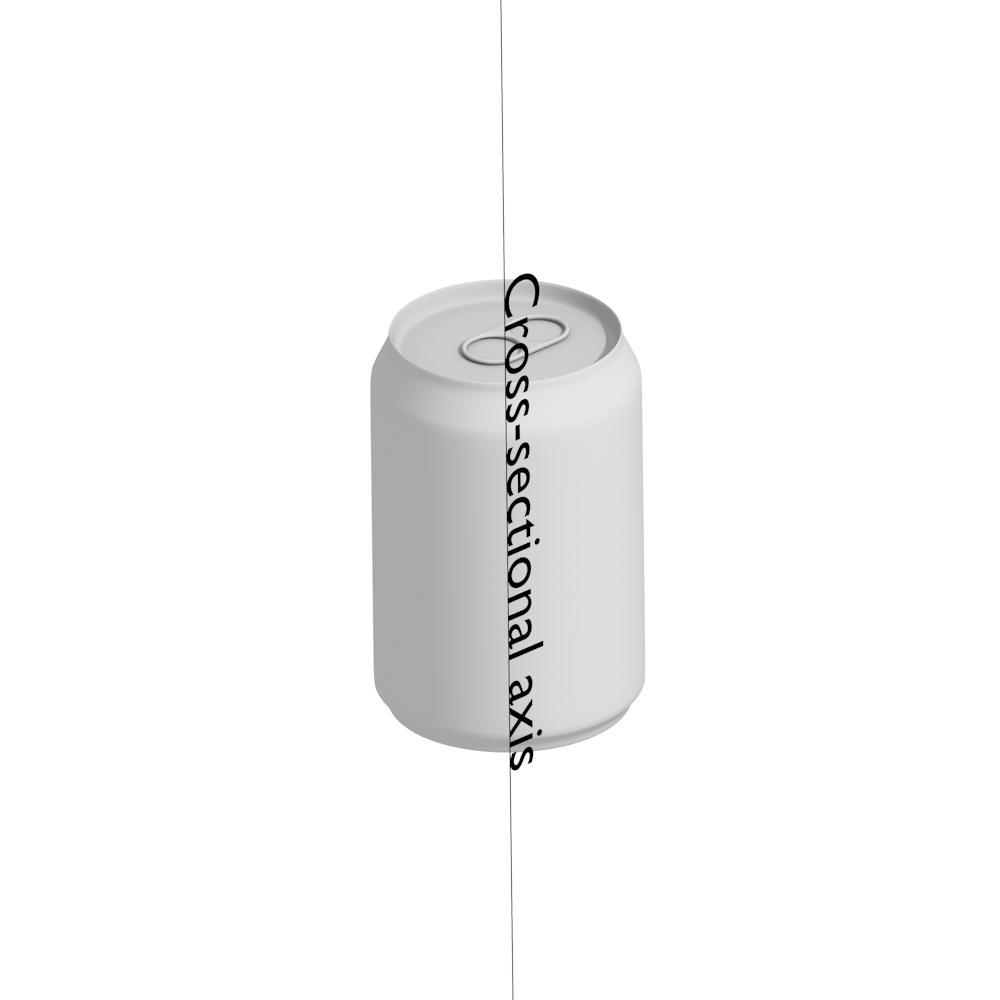
\includegraphics{sodacan.png}
        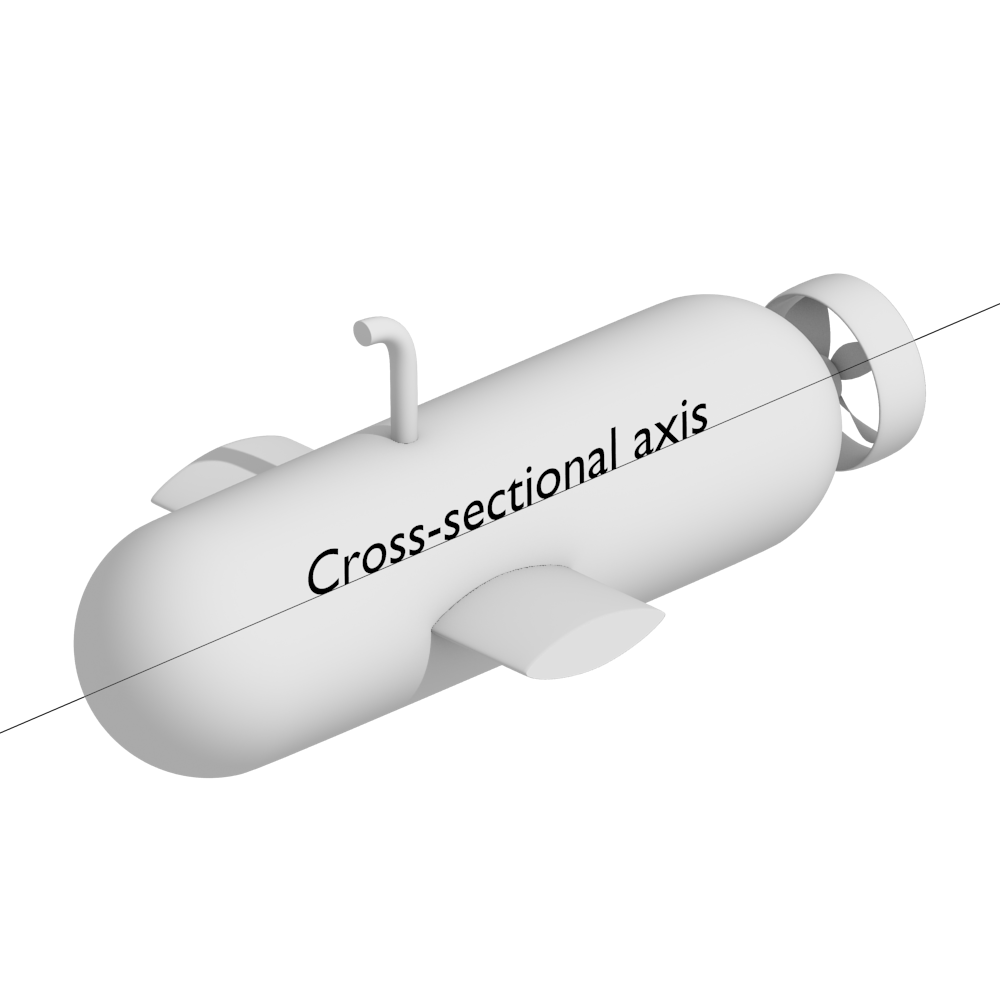
\includegraphics{submarine.png}
    }\caption{Salient Cross-sectional Axes}
    \label{fig:c-sec_axes}
\end{figure}

% paragraph c_sec_axis (end)

% subsubsection spatial_entity_attributes (end)

\subsubsection{Spatial Entity Examples} % (fold)
\label{ssub:spatial_entity_examples}

\textsc{spatial\_entity} tag extents have been identified in \Cref{ex:spatial_entity} followed by pseudo-XML annotations for each tag's attributes have been provided.\footnote{The symbol $\varnothing$ is used in these examples to explicitly indicate an empty, or unspecified value.}

\eenumsentence{
    \item On the large \entity{table}{1} stands a lighted \entity{lamp}{2}.     \vspace{0.5em}\\   
        \textsc{spatial\_entity}
            (\texttt{id}=\texttt{se1},
            \texttt{dimensionality}=\textsc{volume},
            \texttt{mod}=``large'',
            \texttt{line\_type}=$\varnothing$,
            \texttt{area\_type}=\textsc{4-gon},
            \texttt{volume\_type}=\textsc{rect\_prism},
            \texttt{left\_right}=\textsc{relative},\\
            \texttt{front\_back}=\textsc{relative},
            \texttt{top\_bottom}=\textsc{intrinsic},
            \texttt{c-sec\_axis}=\textsc{top\_bottom})\vspace{0.5em}\\
        \textsc{spatial\_entity}
            (\texttt{id}=\texttt{se2},
            \texttt{dimensionality}=\textsc{volume},
            \texttt{mod}=$\varnothing$,
            \texttt{line\_type}=$\varnothing$,\\
            \texttt{area\_type}=\textsc{disc},
            \texttt{volume\_type}=\textsc{cylinder},
            \texttt{left\_right}=\textsc{relative},\\
            \texttt{front\_back}=\textsc{relative},
            \texttt{top\_bottom}=\textsc{intrinsic},
            \texttt{c-sec\_axis}=\textsc{top\_bottom})
        \label{ex:table_lamp}
    \item \entity{}{0} Lies down on \entity{sofa}{3}.
        \begin{note}
            In this example, \texttt{se0} is a non-consuming \textsc{spatial\_entity} tag that is configured relative to the \emph{sofa}.
        \end{note}
        \textsc{spatial\_entity}
            (\texttt{id}=\texttt{se0},
            \texttt{dimensionality}=\textsc{volume},
            \texttt{mod}=$\varnothing$,
            \texttt{line\_type}=$\varnothing$,\\
            \texttt{area\_type}=$\varnothing$,
            \texttt{volume\_type}=$\varnothing$,
            \texttt{left\_right}=$\varnothing$,
            \texttt{front\_back}=$\varnothing$,\\
            \texttt{top\_bottom}=\textsc{intrinsic},
            \texttt{c-sec\_axis}=\textsc{top\_bottom})\vspace{0.5em}\\
        \textsc{spatial\_entity}
            (\texttt{id}=\texttt{se3},
            \texttt{dimensionality}=\textsc{volume},
            \texttt{mod}=$\varnothing$,
            \texttt{line\_type}=$\varnothing$,\\
            \texttt{area\_type}=\textsc{4-gon},
            \texttt{volume\_type}=\textsc{rect\_prism},
            \texttt{left\_right}=\textsc{intrinsic},\\
            \texttt{front\_back}=\textsc{intrinsic},
            \texttt{top\_bottom}=\textsc{intrinsic},
            \texttt{c-sec\_axis}=\textsc{left\_right})
        \label{ex:sofa}
	\item \entity{MAURICE}{4} and \entity{HENRIETTE}{5} are in evening dress and sit facing each other \ldots\vspace{0.5em}\\
        \textsc{spatial\_entity}
            (\texttt{id}=\texttt{se4},
            \texttt{dimensionality}=\textsc{volume},
            \texttt{mod}=$\varnothing$,
            \texttt{line\_type}=$\varnothing$,\\
            \texttt{area\_type}=$\varnothing$,
            \texttt{volume\_type}=\textsc{biped},
            \texttt{left\_right}=\textsc{intrinsic},
            \texttt{front\_back}=\textsc{intrinsic},
            \texttt{top\_bottom}=\textsc{intrinsic},
            \texttt{c-sec\_axis}=\textsc{top\_bottom})\vspace{0.5em}\\
        \textsc{spatial\_entity}
            (\texttt{id}=\texttt{se5},
            \texttt{dimensionality}=\textsc{volume},
            \texttt{mod}=$\varnothing$,
            \texttt{line\_type}=$\varnothing$,\\
            \texttt{area\_type}=$\varnothing$,
            \texttt{volume\_type}=\textsc{biped},
            \texttt{left\_right}=\textsc{intrinsic},
            \texttt{front\_back}=\textsc{intrinsic},
            \texttt{top\_bottom}=\textsc{intrinsic},
            \texttt{c-sec\_axis}=\textsc{top\_bottom})        
        \label{ex:maurice_henriette}
    \item In the foreground a \entity{table}{6} is spread, with \entity{flowers}{7} in the centre, \entity{bowls}{8} full of \entity{fruit}{9}, \entity{wine}{10} in \entity{decanters}{11}, \entity{oysters}{12} on \entity{platters}{13} \ldots\vspace{0.5em}\\
        \textsc{spatial\_entity}
            (\texttt{id}=\texttt{se6},
            \texttt{dimensionality}=\textsc{volume},
            \texttt{mod}=$\varnothing$,
            \texttt{line\_type}=$\varnothing$,\\
            \texttt{area\_type}=\textsc{4-gon},
            \texttt{volume\_type}=\textsc{rect\_prism},
            \texttt{left\_right}=\textsc{relative},\\
            \texttt{front\_back}=\textsc{relative},
            \texttt{top\_bottom}=\textsc{intrinsic},
            \texttt{c-sec\_axis}=\textsc{top\_bottom})\vspace{0.5em}\\
        \textsc{spatial\_entity}
            (\texttt{id}=\texttt{se7},
            \texttt{dimensionality}=\textsc{volume},
            \texttt{mod}=$\varnothing$,
            \texttt{line\_type}=$\varnothing$,\\
            \texttt{area\_type}=$\varnothing$,
            \texttt{volume\_type}=\textsc{other},
            \texttt{left\_right}=\textsc{relative},\\
            \texttt{front\_back}=\textsc{relative},
            \texttt{top\_bottom}=\textsc{intrinsic},
            \texttt{c-sec\_axis}=\textsc{top\_bottom})\vspace{0.5em}\\
        \textsc{spatial\_entity}
            (\texttt{id}=\texttt{se8},
            \texttt{dimensionality}=\textsc{volume},
            \texttt{mod}=$\varnothing$,
            \texttt{line\_type}=$\varnothing$,\\
            \texttt{area\_type}=\textsc{disc},
            \texttt{volume\_type}=\textsc{other},
            \texttt{left\_right}=\textsc{relative},\\
            \texttt{front\_back}=\textsc{relative},
            \texttt{top\_bottom}=\textsc{intrinsic},
            \texttt{c-sec\_axis}=\textsc{top\_bottom})\vspace{0.5em}\\
        \textsc{spatial\_entity}
            (\texttt{id}=\texttt{se9},
            \texttt{dimensionality}=\textsc{volume},
            \texttt{mod}=$\varnothing$,
            \texttt{line\_type}=$\varnothing$,\\
            \texttt{area\_type}=$\varnothing$,
            \texttt{volume\_type}=\textsc{other},
            \texttt{left\_right}=\textsc{relative},\\
            \texttt{front\_back}=\textsc{relative},
            \texttt{top\_bottom}=\textsc{relative},
            \texttt{c-sec\_axis}=$\varnothing$)\vspace{0.5em}\\
        \textsc{spatial\_entity}
            (\texttt{id}=\texttt{se10},
            \texttt{dimensionality}=\textsc{volume},
            \texttt{mod}=$\varnothing$,
            \texttt{line\_type}=$\varnothing$,\\
            \texttt{area\_type}=$\varnothing$,
            \texttt{volume\_type}=\textsc{other},
            \texttt{left\_right}=\textsc{relative},\\
            \texttt{front\_back}=\textsc{relative},
            \texttt{top\_bottom}=\textsc{relative},
            \texttt{c-sec\_axis}=$\varnothing$)\vspace{0.5em}\\
        \textsc{spatial\_entity}
            (\texttt{id}=\texttt{se11},
            \texttt{dimensionality}=\textsc{volume},
            \texttt{mod}=$\varnothing$,
            \texttt{line\_type}=$\varnothing$,\\
            \texttt{area\_type}=\textsc{disc},
            \texttt{volume\_type}=\textsc{other},
            \texttt{left\_right}=\textsc{relative},\\
            \texttt{front\_back}=\textsc{relative},
            \texttt{top\_bottom}=\textsc{intrinsic},
            \texttt{c-sec\_axis}=\textsc{top\_bottom})\vspace{0.5em}\\
        \textsc{spatial\_entity}
            (\texttt{id}=\texttt{se12},
            \texttt{dimensionality}=\textsc{volume},
            \texttt{mod}=$\varnothing$,
            \texttt{line\_type}=$\varnothing$,\\
            \texttt{area\_type}=$\varnothing$,
            \texttt{volume\_type}=\textsc{other},
            \texttt{left\_right}=\textsc{intrinsic},\\
            \texttt{front\_back}=\textsc{intrinsic},
            \texttt{top\_bottom}=\textsc{intrinsic},
            \texttt{c-sec\_axis}=\textsc{top\_bottom})\vspace{0.5em}\\
        \textsc{spatial\_entity}
            (\texttt{id}=\texttt{se13},
            \texttt{dimensionality}=\textsc{volume},
            \texttt{mod}=$\varnothing$,
            \texttt{line\_type}=$\varnothing$,\\
            \texttt{area\_type}=\textsc{disc},
            \texttt{volume\_type}=\textsc{cylinder},
            \texttt{left\_right}=\textsc{relative},\\
            \texttt{front\_back}=\textsc{relative},
            \texttt{top\_bottom}=\textsc{intrinsic},
            \texttt{c-sec\_axis}=\textsc{top\_bottom})\vspace{0.5em}\\
    \label{ex:table_flowers_etc}
}\label{ex:spatial_entity}


% subsubsection spatial_entity_tag_examples (end)

% subsection spatial_entity (end)

\subsection{Orientation Signal Tag} % (fold)
\label{sub:orientation_signal_tag}

An orientation signal is taken to be some word or phrase that restricts the potential configurational interpretations of a spatial entity. Orientation signals always trigger configuration links, so, if an annotator tags a orientation signal, then they are committing to also creating a configuration link.

Sentences in \Cref{ex:non_trigger_examples} have had \textsc{orientation\_signal} extents identified.

\eenumsentence{
    \item On the large table \signal{stands}{1} a lighted lamp.
    \label{ex:lamp_stands}
    \item \signal{Lies}{2} down on sofa.
    \label{ex:lies_sofa}
	\item MAURICE and HENRIETTE are in evening dress and \signal{sit}{3} \signal{facing}{4} each other \ldots
	\label{ex:sit_facing}
	\item In the foreground a table is spread, with flowers in the centre, bowls full of fruit, wine in decanters, oysters on platters \ldots
	\label{ex:foreground_table}
}\label{ex:non_trigger_examples}

Here, in \Cref{ex:lamp_stands}, the signal \emph{stands} serves to adumbrate in what configuration the lamp is arranged individually. Because the lamp \emph{stands} rather than, e.g., \emph{lies} or \emph{leans}, one immediately recognizes that the lamp is situated in such a way that its top-bottom axis is aligned vertically.

Likewise, in \Cref{ex:lies_sofa}, the signal \emph{lies} indicates that some entity---in this case an implicit spatial entity, which would need to be created via a non-consuming \textsc{spatial\_entity} tag---is configured in such a way that its top-bottom orientational axis is horizontally aligned. 

\iffalse
Examples of the latter type are enumerated in \Cref{ex:trigger_examples}.

\eenumsentence{
	\item MAURICE and HENRIETTE are in evening dress and sit facing each other \ldots
	\label{ex:sit_facing}
	\item In the foreground a table is spread, with flowers in the centre, bowls full of fruit, wine in decanters, oysters on platters \ldots
	\label{ex:foreground_table}
}\label{ex:trigger_examples}

%In the foreground a table is spread, with flowers [in] the [centre], bowls [full] of fruit, wine [in] decanters, oysters [on] platters ...; I am not sure about the annotation of "in the centre" above, "full of," or "on" above. I am going to leave this explanation blank for the moment.
\fi

\subsubsection{Orientation Signal Extents} % (fold)
\label{ssub:orientation_signal_extents}
% Explain what kinds of lexical items should be captured with the orientation signal tag here.
In general, whereas \textsc{spatial\_entity} terms will be nominals, \textsc{orientation\_signal} terms will belong to other parts of speech, e.g., verbs, prepositions, adjectives, and adverbs. The extent for orientation signals should consist of the head of the phrase, so for phrasal verbs, take only the head verb as the extent for the orientation signal, ignoring any particles. For prepositional phrases, only the head preposition would be tagged.

% subsubsection orientation_signal_extents (end)

\subsubsection{Orientation Signal Attributes} % (fold)
\label{ssub:orientation_signal_attributes}

The orientation signal tag has one attribute that annotators need to consider, as shown in \cref{tab:orientation_signal}:

\begin{table}[h]
\centering
\begin{attributes}
    \hline \texttt{id}                  & \texttt{os1}, \texttt{os2}, 
                                          \texttt{os3}, \ldots\\
    \hline \texttt{orientation\_type}   & \textsc{latitudinal}, 
                                          \textsc{longitudinal}, 
                                          \textsc{lateral}, \textsc{vertical}, 
                                          \textsc{other}\\
\end{attributes}
\caption{Attributes for \textsc{orientation\_signal}}
\label{tab:orientation_signal}
\end{table}

\paragraph{\texttt{orientation\_type}} % (fold)
\label{par:orientation_type}
The \texttt{orientation\_type} attribute specifies an axis of orientation that is accessed by the orientation signal. The \textsc{latitudinal} value refers to the left-right axis, the \textsc{longitudinal} to the front-back axis, and the \textsc{vertical} to the top-bottom axis. The \textsc{lateral} value is supplied to capture cases in which a horizontal axis is accessed, yet there is no distinction between the left-right and the front-back axes. The value of \textsc{other} should be selected for such cases as specify a configuration not covered by the remaining values.

% Go through each attribute, in depth, here.

% subsubsection other_tag_attributes (end)

\subsubsection{Orientation Signal Examples} % (fold)
\label{ssub:orientation_signal_examples}

Provided below, in \Cref{ex:orientation_signals}, are sample annotations for extents to be tagged as \textsc{orientation\_signal}:

\eenumsentence{
    \item On the large table \signal{stands}{1} a lighted lamp.
    \label{ex:annot_stands}
    \item \ldots \signal{lies}{2} down on sofa.
    \label{ex:annot_lies}
    \item MAURICE and HENRIETTE are in evening dress and \signal{sit}{3} \signal{facing}{4} each other \ldots
	\label{ex:annot_sit_facing}
	\item In the foreground a table is spread, with flowers \signal{in}{5} the centre, bowls \signal{full}{6} of fruit, wine \signal{in}{7} decanters, oysters \signal{on}{8} platters \ldots
	\label{ex:annot_table}
}\label{ex:orientation_signals}

% What about [spread]? Would we want to capture it differently if the sentence said [stacked] instead of [spread]?

% We need to talk about how we are not actually capturing containment relations. E.g, for \emph{fruit in the bowl} and \emph{wine in decanters}, the $contains{container,containee}$ is a topological relation, distinct from the orientation relations we are capturing with configuration links, though there may be some conflation of the two. ISO-Space classifies \textsc{spatial\_signal} tags as topological, orientational, or both, but since OCDML is focused strictly on orientation, the cases where conflation does occur are going to be difficult.

% subsubsection orientation_signal_examples (end)

% subsection orientation_signal_tag (end)

% section extent_tags (end)

\section{Link Tags} % (fold)
\label{sec:link_tags}

\subsection{Configuration Link Tag} % (fold)
\label{sub:configuration_link}
The \textsc{configuration\_link} relates two \textsc{spatial\_entity} tags. For each \textsc{configuration\_link}, one \textsc{spatial\_entity} will be referred to as the figure in the relation, and the other will be referred to as the ground. The figure is the spacial entity that moves or is located in relation to the ground. Similarly, the ground is the spacial entity against which the figure moves, or in relation to which the figure is located. In \Cref{ex:cat}, \emph{cat} is the figure and \emph{table} is the ground, since the \emph{cat} is located in relation to the \emph{table}. In \Cref{ex:man}, \emph{man} is the figure and \emph{street} is the ground, since the \emph{man} is moving in relation to the \emph{street}. The figure is typically the smaller, more movable object, but this is not always the case, as can be seen in \Cref{ex:house}. In English, the figure tends to come before the ground in the sentence. While this is a helpful heuristic, it should not be the sole basis of your annotation decisions, as is evident from \Cref{ex:lady}.
 
% Cynthia: When creating the link, always link from the figure to the ground? This is related to my question about the direction attribute.

\eenumsentence{
    \item The [cat$_{figure}$] is sitting on the [table$_{ground}$].
    \label{ex:cat}
    \item The [man$_{figure}$] walked down the [street$_{ground}$].
    \label{ex:man}
    \item The [house$_{figure}$] landed on the [witch$_{ground}$].
    \label{ex:house}
    \item \ldots sitting at the [desk$_{ground}$] was a beautiful [woman$_{figure}$].
    \label{ex:lady}
}\label{ex:fig_ground_examples}


% subsection configuration_link (end)


\subsubsection{Configuration Link Attributes} % (fold)
\label{ssub:configuration_link_attributes}

The attributes for the \textsc{configuration\_link} tag are enumerated in \cref{tab:configuration_link}. 

\begin{table}[h]
\centering
\begin{attributes}
    \hline \texttt{id}                  & \texttt{cl1}, \texttt{cl2}, 
                                          \texttt{cl3}, \ldots\\
    \hline \texttt{figure\_config}      & \textsc{left}, \textsc{right}, \textsc{front}, \textsc{back}, \textsc{top}, \textsc{bottom}, \textsc{side}, \textsc{top\_or\_bottom}, \textsc{any}, \textsc{other}\\
    \hline \texttt{ground\_config}      & \textsc{left}, \textsc{right}, \textsc{front}, \textsc{back}, \textsc{top}, \textsc{bottom}, \textsc{side}, \textsc{top\_or\_bottom}, \textsc{any}, \textsc{other}\\
    \hline \texttt{coercion}            & \textsc{figure}, \textsc{ground}, or \textsc{none}\\
    \hline \texttt{trigger}             & An ID of a \texttt{orientation\_signal} tag that triggers the link\\
    \hline \texttt{direction}           & \textsc{figure\_ground}, \textsc{ground\_figure}\\
\end{attributes}
\caption{Attributes for \textsc{configuration\_link}}
\label{tab:configuration_link}
\end{table}

% Zach: I added \textsc{side}, \textsc{top\_or\_bottom} and \textsc{any} configuration values to handle cases where the configuration is only partly specified, e.g., ``Lies on the couch.'', where is the the implicit figure's \textsc{side} that is related to the \textsc{top} of the couch. We also need the \textsc{any} value for ``fruit in the bowl'', where we take the fruit to be the figure, and it is fruit's \textsc{any} being related to the bowl's \textsc{bottom}.

\paragraph{\texttt{figure\_config} \& \texttt{ground\_config}} % (fold)
\label{par:figure_ground_config}
The combination of the \texttt{figure\_config} and \texttt{ground\_config} attributes are used to specify the configuration between the participating figure and ground entities. 

\iffalse
Looking back at \Cref{ex:cat}, the configuration of the entities involved is such that the bottom of the cat is on the top of the table. The \texttt{figure\_config} attribute is compulsory whereas the ground config attribute is optional; \Cref{ex:ground} shows an optional \texttt{ground\_config} whereas in \Cref{ex:no_ground} the \texttt{ground\_config} is requisite.

% Zach: I don't agree with this. We need to be able to handle cases where there is a lot of underspecification.
\fi

\eenumsentence{
    \item The [cat$_{figure}$] is sitting on the [table$_{ground}$].
    \label{ex:ground}
    \item The [cat$_{figure}$] is sitting alone [$_{ground}$].
    \label{ex:no_ground}
}\label{ex:ground_requirement}

% paragraph figure_ground_config (end)

\paragraph{\texttt{dim\_coercion}} % (fold)
\label{par:dim_coercion}

This attribute can be used to indicate that the dimensionality of the figure entity is coerced to that of the ground or vice versa. Consider \Cref{ex:sun}. While we know that the sun is a 3-dimensional sphere, in this example the \emph{sun} is being coerced into 2-dimensions by the ground, namely the \emph{sky}. This type of coercion does not take place in \Cref{ex:earth}, since both the \emph{earth} and the \emph{sun} would be considered 3-dimensional objects moving in 3-dimensional space.

\eenumsentence{
    \item The [sun$_{figure}$] travels across the [sky$_{ground}$].
    \label{ex:sun}
    \item The [earth$_{figure}$] rotates around the [sun$_{ground}$].
    \label{ex:earth}
}\label{ex:coercion}

% Zach: @Cynthia, nice examples!

% paragraph dim_coercion (end)

\paragraph{\texttt{trigger}} % (fold)
\label{par:trigger}
This attribute takes the ID value of the \texttt{orientation\_signal} that triggered the \texttt{configuration\_link}. Recall that creating an \texttt{orientation\_signal} means committing to creating a \textsc{configuration\_link}, however, there may be situations where a \textsc{configuration\_link} is created without any triggering signal.

% Zach: We should add some xamples for the latter case, if not here, then in our fully annotated examples section. 

    % In the foreground a \entity{table}{6} is spread, with \entity{flowers}{7} in the centre, \entity{bowls}{8} full of \entity{fruit}{9}, \entity{wine}{10} in \entity{decanters}{11}, \entity{oysters}{12} on \entity{platters}{13}

    % This is one example where we would want to have links between [bowls] and [table], [decanters] and [table], and [platters] and [table], even though there are no explicit signals for these relations, right?

% paragraph trigger (end)

\paragraph{\texttt{direction}} % (fold)
\label{par:direction}
This attribute is used to indicate the asymmetrical directionality of the configuration relation in terms of figure-to-ground or ground-to-figure. When creating a \textsc{configuration\_link}, if the ID of the \textsc{spatial\_entity} tag that represents the figure is selected first, then the \texttt{direction} attribute should take a value of \textsc{figure\_ground}. If the link were created in the reverse order, such that the ID of the \textsc{spatial\_entity} tag that represents the ground is selected first, then the \texttt{direction} attribute should take a value of \textsc{ground\_figure}.
%Cynthia: remind me again why we decided to use this instead of specifying that the annotator always tag the figure first and the ground second, regardless of word order? I thought we had decided to do the latter, but now I'm unsure. How would we annotate the sentence "… and sitting in the chair was a beautiful lady"?

% Zach: @Cynthia, the problem with relying on the order of the link creation is that it's relying on the annotators to remember the correct order, whereas allowing the order to be switched, but having explicit figure and ground attributes is more flexible for the annotators and less prone to mistakes being made, since annotators must be explicit about which entity ID is the figure and which is the ground.

% paragraph direction (end)



% subsubsection configuration_link_attributes (end)
% section link_tags (end)

\section{Fully Annotated Examples} % (fold)
\label{sec:fully_annotated_examples}

% List some full annotation sample sentences and pseudo-XML annotations along with discussion of the motivations for any decisions which were made.

% Zach: We need examples that explain the choices that need to be made:
    % How do we tag pronouns like [other] and [another], [each other] etc.?
    % 


% section fully_annotated_examples (end)

\section{Phased Annotation Approach} % (fold)
\label{sec:phased_annotation_approach}

For this task we will be dividing the annotation into three sections as enumerated in the outline below. This phased approach is intended to establish a consistent set of entity and signal extent tags early in the process. For the first annotation phase, annotators will simply be identifying \textsc{spatial\_entity} and \textsc{spatial\_signal} tag extents. After the first annotation phase, a cursory round of adjudication will be performed in order to lock in a consistent set of extent tags. Once this consistent set of extents has been frozen, annotators will fill the attributes for those extent tags. Finally, during the third phase of annotation, annotators will create the links between the locked set of extent tags. After the third annotation phase the final adjudication will occur.

\begin{description}
    \item[Annotation Phase 1] Extents for \textsc{spatial\_entity} and \textsc{orientation\_signal} tags.
    \item[Extents Adjudication] Extent tags will be adjudicated and locked.
    \item[Annotation Phase 2] Attributes for locked \textsc{spatial\_entity} and \textsc{orientation\_signal} tags.
    \item[Annotation Phase 3] Creation of \textsc{configuration\_links} annotation of link attributes.
    \item[Final Adjudication] Link tags and all tag attributes will be adjudicated.
\end{description}
\label{desc:phases}


% section phased_annotation_approach (end)
\end{document}